\documentclass[11pt, a4paper]{article}

% Packages
\usepackage[english]{babel}
\usepackage[T1]{fontenc}
\usepackage[utf8]{inputenc}

\usepackage[left=2cm, right=2cm, top=2cm, bottom=2cm]{geometry}
\usepackage{fancyhdr}
\usepackage{lastpage}
\usepackage{hyperref}

\usepackage{float}

\usepackage{graphicx}
\graphicspath{{./img/}}

\usepackage{pgfplots}
\pgfplotsset{compat=1.13}

\usepackage{listings}

\usepackage{csvsimple}

\usepackage{color}
% Listings --------------------------------------------------------------------
\lstset{
    basicstyle=\ttfamily\small,
    stringstyle=\ttfamily\color{green!50!black},
    keywordstyle=\bfseries\color{blue},
    commentstyle=\itshape\color{red!50!black},
    showstringspaces=true,
    tabsize=4,
    frame=single,
    numberstyle=\tiny,
    firstnumber=1,
    stepnumber=1,
    numbersep=5pt,
    breaklines=true
}

% Reset paragraph indentation -------------------------------------------------
\setlength{\parindent}{0cm}

% Allow a paragraph to have a linebreak ---------------------------------------
\newcommand{\paragraphnl}[1]{\paragraph{#1}\mbox{}\\}

% PGF plot table key ----------------------------------------------------------
% http://tex.stackexchange.com/questions/84541/simpler-boxplots-in-pgfplots-is-this-possible
\pgfplotsset{
    box plot/.style={
        /pgfplots/.cd,
        black,
        only marks,
        mark=-,
        mark size=\pgfkeysvalueof{/pgfplots/box plot width},
        /pgfplots/error bars/y dir=plus,
        /pgfplots/error bars/y explicit,
        /pgfplots/table/x index=\pgfkeysvalueof{/pgfplots/box plot x index},
    },
    box plot box/.style={
        /pgfplots/error bars/draw error bar/.code 2 args={%
            \draw  ##1 -- ++(\pgfkeysvalueof{/pgfplots/box plot width},0pt) |- ##2 -- ++(-\pgfkeysvalueof{/pgfplots/box plot width},0pt) |- ##1 -- cycle;
        },
        /pgfplots/table/.cd,
        y index=\pgfkeysvalueof{/pgfplots/box plot box top index},
        y error expr={
            \thisrowno{\pgfkeysvalueof{/pgfplots/box plot box bottom index}}
            - \thisrowno{\pgfkeysvalueof{/pgfplots/box plot box top index}}
        },
        /pgfplots/box plot
    },
    box plot top whisker/.style={
        /pgfplots/error bars/draw error bar/.code 2 args={%
            \pgfkeysgetvalue{/pgfplots/error bars/error mark}%
            {\pgfplotserrorbarsmark}%
            \pgfkeysgetvalue{/pgfplots/error bars/error mark options}%
            {\pgfplotserrorbarsmarkopts}%
            \path ##1 -- ##2;
        },
        /pgfplots/table/.cd,
        y index=\pgfkeysvalueof{/pgfplots/box plot whisker top index},
        y error expr={
            \thisrowno{\pgfkeysvalueof{/pgfplots/box plot box top index}}
            - \thisrowno{\pgfkeysvalueof{/pgfplots/box plot whisker top index}}
        },
        /pgfplots/box plot
    },
    box plot bottom whisker/.style={
        /pgfplots/error bars/draw error bar/.code 2 args={%
            \pgfkeysgetvalue{/pgfplots/error bars/error mark}%
            {\pgfplotserrorbarsmark}%
            \pgfkeysgetvalue{/pgfplots/error bars/error mark options}%
            {\pgfplotserrorbarsmarkopts}%
            \path ##1 -- ##2;
        },
        /pgfplots/table/.cd,
        y index=\pgfkeysvalueof{/pgfplots/box plot whisker bottom index},
        y error expr={
            \thisrowno{\pgfkeysvalueof{/pgfplots/box plot box bottom index}}
            - \thisrowno{\pgfkeysvalueof{/pgfplots/box plot whisker bottom index}}
        },
        /pgfplots/box plot
    },
    box plot median/.style={
        /pgfplots/box plot,
        /pgfplots/table/y index=\pgfkeysvalueof{/pgfplots/box plot median index}
    },
    box plot width/.initial=1em,
    box plot x index/.initial=0,
    box plot median index/.initial=1,
    box plot box top index/.initial=2,
    box plot box bottom index/.initial=3,
    box plot whisker top index/.initial=4,
    box plot whisker bottom index/.initial=5,
}

\newcommand{\boxplot}[2][]{
    \addplot [box plot median,#1] table {#2};
    \addplot [forget plot, box plot box,#1] table {#2};
    \addplot [forget plot, box plot top whisker,#1] table {#2};
    \addplot [forget plot, box plot bottom whisker,#1] table {#2};
}

% Page header and footer ------------------------------------------------------
\pagestyle{fancy}
\setlength{\headheight}{33pt}
\renewcommand{\headrulewidth}{0.5pt}
\lhead{
\includegraphics[height=1cm]{hepia.jpg}}
\chead{Cracker de mot de passe}
\rhead{Claudio Sousa - David Gonzalez}
\renewcommand{\footrulewidth}{0.5pt}
\lfoot{1 novembre 2016}
\cfoot{}
\rfoot{Page \thepage /\pageref{LastPage}}

% Table of contents depth -----------------------------------------------------
\setcounter{tocdepth}{3}

% Document --------------------------------------------------------------------
\begin{document}

\title
{
    \Huge{Programmation concurrente} \\
    \Huge{Password Cracker}
}
\author
{
	\LARGE{Claudio Sousa - David Gonzalez}
}
\date{1 novembre 2016}
\maketitle

\vspace{50pt}

\begin{center}
    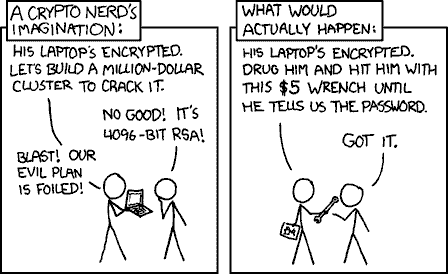
\includegraphics[scale=.8]{frontpage.png}
\end{center}

\thispagestyle{empty}

\newpage

% -----------------------------------------------------------------------------
\section{Introduction}
\subsection{Division des tâches}
Chaque membre du group a fait seul le programme dans son entièreté. Le travail rendu est la mise en commun du code des differents programmes.

\subsection{Machine cible}
\textbf{lscpu:}
\begin{lstlisting}
Architecture:          x86_64
CPU op-mode(s):        32-bit, 64-bit
Byte Order:            Little Endian
CPU(s):                8
On-line CPU(s) list:   0-7
Thread(s) per core:    2
Core(s) per socket:    4
Socket(s):             1
NUMA node(s):          1
Vendor ID:             GenuineIntel
CPU family:            6
Model:                 60
Stepping:              3
CPU MHz:               800.000
BogoMIPS:              7183.36
Virtualization:        VT-x
L1d cache:             32K
L1i cache:             32K
L2 cache:              256K
L3 cache:              8192K
NUMA node0 CPU(s):     0-7
\end{lstlisting}



% -----------------------------------------------------------------------------
\section{Thread performance comparison}
\subsection{Méthodologie}
Afin de produire les données statistiques de performance, le cracker a été modifié afin de s'éxécuter pendant 10s et imprimer le nombre de mot de passes encryptées par seconde.
20 testes ont été fais pour chaque nombre de threads utilisé  (2\textsuperscript{\{0..8\}})


\subsection{Données}

\begin{figure}[H]
    \begin{center}
        \begin{tikzpicture}
            \begin{semilogxaxis}[
                    width=1.0\textwidth,
                    xtick=data,
                    log ticks with fixed point,
                    x tick label style={/pgf/number format/1000 sep=\,},
                    xlabel=Nombre de threads,
                    ylabel=10 \textsuperscript{6} pwds/s,
                   %yscale=.9
                ]
                \boxplot[forget plot, fill=lightgray] {data/threads.csv};
                \addplot[color=gray,fill=white,mark=*,only marks] table[x index=0,y index=1]{data/threads_outlayer.csv};
            \end{semilogxaxis}
        \end{tikzpicture}
    \end{center}
    \caption{Comparaison des performances avec un nombre différent de threads}
    \label{Comparaison des performances avec un nombre différent de threads}
\end{figure}



\begin{table}[H]
	\begin{center}
		\csvreader[
		separator=tab,
		no head,
		tabular=|l|l|l|l|l|l|,
		table head=\hline \textbf{Nombre de threads} & \textbf{Median} & \textbf{Q3} & \textbf{Q1} & \textbf{Q4} & \textbf{Q0} \\\hline\hline,
		late after line=\\\hline
		]
		{data/threads.csv}{}
		{\csvcoli & \csvcolii & \csvcoliii & \csvcoliv & \csvcolv & \csvcolvi}
	\end{center}
	\caption{Comparaison des performances avec un nombre différent de threads}
	\label{Comparaison des performances avec un nombre différent de threads}
\end{table}


\newpage
\subsection{Questions \& réponses}
\paragraphnl{Le gain de vitesse est linéaire avec le nombre de threads?}
Le gain de performance (mots de pass crackés par second) avec le nombre de threads est essentiellement linéaire (on ne double pas, mais presque) jusqu'au nombre de CPUs logiques sur la machine hôte. \\

L'utilisation de threads supplémentaires n'augmente pas la performance. Au contraire, la performance diminue. 
En effet, si nous avons déjà un thread par CPU logique, nous avons déjà un taux d'utilisation de 100\% pour chaque CPUs. Augmenter alors le nombre de threads utilisé ne permettra pas d'augmenter le taux d'utilisation des CPUs, et créera inévitablement une baisse de performance due au temps passé à changer de contexte.\\


\begin{figure}[H]
	\begin{center}
		\begin{tikzpicture}
			\begin{axis}[
				 xlabel=Nombre de threads,
				 ylabel=10 \textsuperscript{6} pwds/s,
				xtick={1,2, 4, 8},
				xmajorgrids=true,
				grid style=dashed
			]
			\addplot[
				color=blue,
				mark=square,
			]
			coordinates {
				(1, 0.421)(2,0.834 )( 4, 1.433)( 8, 2.089)
			};
			\end{axis}
		\end{tikzpicture}
	\end{center}
    \caption{Comparison de la performance par thread avec axe des abscisses avec échelle linéaire}
    \label{Comparison de la performance par thread avec axe des abscisses avec échelle linéaire}
\end{figure}

\paragraphnl{Quel est l'impact de l'hyper-threading sur les performances?}
Le hyper-threading permet de doubler le nombre de CPUs. Dans notre cas, malgré que la machine n'ait que 4 CPUs physiques, l'hyper-threading permet d'avoir 8 CPUs logiques à disposition. \\

Chaque CPU logique possède son propre jeu de registres, mais la paire partage la même unité de calcul. Nous avons pu constater empiriquement que la ressource partagée entre chaque paire de CPUs logiques (l'ALU) ne semble pas être utilisée dans sa totalité par un seul CPU logique. En effet, l'utilisation du 2\textsuperscript{ème} CPU logique (sur le même CPU physique) permet, d'après nos résultats, de quasiment doubler les performances.
 
\paragraphnl{Mot de passe trouvé}
groumf (après 2h20m53s)
\end{document}
